\chapter{Background}\label{ch:background}
\glsresetall
This chapter introduces the technical foundations required to understand gradient-based parameter fitting in simplified neuron models.
We start with the \gls{AdEx} model and explain why its parameters need to be fitted (Section~\ref{sec:bg:neuron-models}).
We then discuss the landscape of parameter tuning methods, motivating why gradient-based approaches are attractive but face a fundamental obstacle:
the non-differentiable reset mechanism (Section~\ref{sec:bg:parameter-tuning}).
Surrogate gradients overcome this obstacle, but introduce their own challenges --- vanishing gradients through leak dynamics and sensitivity to the surrogate shape (Section~\ref{sec:bg:surrogate-gradients}).
Finally, even with working gradients, the loss function determines whether optimisation succeeds.
We survey three categories of loss functions and their trade-offs for spiking models (Section~\ref{sec:bg:loss-functions}).

\section{Neuron Models}\label{sec:bg:neuron-models}
Large-scale brain models are limited in size mostly by computational feasibility.
Detailed bio-physical models which combine multi-compartment reconstructions of neuron morphology
with non-linear ion channel dynamics (\gls{HH}, stochastic models)
can precisely predict membrane behaviour of a vast variety of neuron types.
However, they require huge computational resources to estimate the required parameters to fit the models to experimental data.
Simplified Neuron Models overcome this challenge, capturing a subset of the sophisticated neuron behaviour with only a fraction of the computational cost, enabling large-scale simulations \cite{Gerstner2014}.
Point neuron models boost computational performance by reducing branched neuron morphologies to a single active compartment.
The \gls{AdEx} model \cite{Naud2008} provides a particularly interesting balance --- it reproduces a variety of firing patterns but drastically reduces the number of necessary parameters of the model.
This makes it a favourable model for large-scale neuron simulations \cite{Tesler2024}.

The \gls{AdEx} model improves the simpler \gls{LIF} model in two ways:
first, it introduces exponential behaviour when initialising the spike.
Second, the model allows for adaptation, meaning it can change spiking frequencies or post-spike refractoriness based on their firing history.
It is defined by the equations given in \cite{Brette2005, Naud2008}:
\begin{align}
  C \frac{dV}{dt} &= -g_L (V - E_L) + g_L \Delta_T \exp(\frac{V - V_T}{\Delta_T}) + I - w,\label{eq:adex1}\\
  \tau_w \frac{dw}{dt} &= a(V - E_L) - w,\label{eq:adex2}
\end{align}
with the following reset condition:
\begin{align}
  \text{if } V > 0 \text{ mV}\; \text{ then} &= \begin{cases}
    V \rightarrow V_r,\\
    w \rightarrow w_r = w + b.
  \end{cases}\label{eq:adex3}
\end{align}

It describes the membrane potential over time $V(t)$ given an injected current $I(t)$.
Equation (\ref{eq:adex1}) describes the change of potential.
$C$ is the membrane capacitance, $g_L$ the leak conductance and $E_L$ the effective resting potential.
We can understand $-g_L (V - E_L)$ as the leak current that slowly pulls the membrane potential towards its resting potential.
$g_L \Delta_T \exp(\frac{V - V_T}{\Delta_T})$ models the depolarisation initialised by the fast reacting sodium channels using an exponential function,
modelled using a driving force based on an effective threshold potential $V_T$ and a slope factor $\Delta_T$.
$I$ is the injected current, and $w$ is the adaptation current, which is described in equation \ref{eq:adex2}.

The adaptation mechanism is controlled via an adaptation current which opposes depolarisation.
Unlike the fast membrane behaviour, this current is related to the time constant $\tau_w$, which controls the decay time.
It is controlled by $a$ (sub-threshold adaptation) as well as $b$ (spike-triggered adaptation).

Even though the number of parameters is significantly reduced compared to bio-physical \gls{HH}-type models, it still requires parameter fitting --- especially because some parameters (e.g. $a$, $b$ or $\tau_w$) do not have direct physiological counterparts (like $C$ or $g_L$).
For \gls{AdEx} to perform as an effective tool, efficient methods for parameter optimizations are essential.

The \gls{AdEx} equations (Eqs.~\ref{eq:adex1},\ref{eq:adex2}) are continuous ordinary differential equations with a singular discontinuity at spike events.
To simulate numerically, we discretise into a series of time steps $t_0, t_1 = t_0 + \Delta t, ..., T$.
Given the state $s_t = (V_t, w_t)$ at time $t$, we compute $s_{t+1}$ using forward Euler for $V$ and exponential Euler for $w$.
This produces a sequence of states $s_0, s_1, ..., s_T$ — the same that \gls{BPTT} (Section~\ref{sec:bg:sg:bptt}) will differentiate through.
It is important to note that both integration method and time step size $\Delta t$ affect both simulation accuracy and gradient quality.

\section{Parameter Tuning for Neuron Models}\label{sec:bg:parameter-tuning}
A central challenge in neuroscience has been to 'identify the parameters of detailed biophysical models, such that they match physiological measurements at scale' \cite{Deistler2025} in reasonable simulation runtimes.
The parameter space is highly non-convex, which is a challenge for any optimisation approach.
We further dive into this problem in Sec.~\ref{sec:bg:loss:param-space}.
The zoo of optimisation techniques is large, spanning from evolutionary algorithms \cite{VanGeit2008} to gradient descent \cite{Jones2024}, however, deciding which algorithm to use may often depend on the underlying properties of the model.
For tuning simplified neuron models, many different approaches have been used.

\subsection{Non-gradient-based Tuning}\label{sec:bg:tuning:non-gradient-based}
Derivative free methods like Nelder-Mead have successfully been used to fit parameters.
It has simple design principles: it maintains a simplex (geometric shape of $n+1$ vertices in $n$ dimensions) and iteratively transforms it through four operations:
reflection, expansion, contraction and shrinkage.
At each step, the worst vertex is replaced by a better point found through these geometric operations.
The simplex adapts its shape to the landscape --- elongating along valleys, shrinking near minima, ending when it becomes sufficiently small.
Parameter optimisation is well-suited in regards to low-dimensionality: neuron models don't have many parameters which is good (~5-12);
however, it's a local optimizer.
Simplex algorithms converge to the nearest minimum from its starting point.
There exist no mechanism to escape local minima in non-convex landscapes, which requires lots of iterations with different starting positions.

A different popular choice are \glspl{EA}:
These models maintain a collection of candidate solutions (population, parameter sets).
At each generation, fitness is evaluated using an objective functions.
Fittest solution 'produces offspring' through mutation and recombination.
Similar to the simplex algorithm, this only requires forward evaluation of the simulator.
Multi-objective variants optimize for several objective functions simultaneously.
This is a useful feature because for neuron fitting, multiple features (spike count, timing, frequencies, subthreshold voltage, ...) extracted from multiple traces can be treated as separate objectives rather than a single objective function.
\glspl{EA} reduce the risk of under-sampling, however, they typically require hundreds to thousands of generations with tens to hundreds of individuals --- that needs lots of computational resources.

Main advantage of these methods is that they are derivative-free: only the forward pass and objective function is evaluated.
This makes them applicable to any model and any metric, including non-differentiable ones.
However, the cost is sample efficiency — each candidate requires a full forward simulation, and many candidates are needed per optimization run.

\subsection{Gradient-based Tuning}\label{sec:bg:tuning:gradient-based}
Gradient-based optimisation requires computing the partial derivative $\partial L / \partial \theta$ for all trainable parameters.
Doing this analytically is impractical and inefficient for complex simulations with thousands of timesteps.
\gls{AD} solves this by decomposing the computation into elementary operations and applying the chain rule\mwarning{Alex underlined this. Should I define the chain rule? Isn't that basic analysis knowledge? What exactly am I missing here.} systematically.
The most common method is reverse-mode \gls{AD}, also called \gls{BP}, is a particularly efficient method:
it creates a computational graph of operations --- each of them has to be differentiable.
Then one backward pass yields all parameter gradients simultaneously.
\texttt{JAX}, a high performance array computing library, implements this through function tracing and transformation (\verb|jax.grad|).

A modern instantiation of this approach is \texttt{Jaxley} \cite{Deistler2025}, a \texttt{JAX}-based simulator that enables gradient-based fitting of \gls{HH}-type biophysical models at scale (\cref{sec:rw:param-estimation:gbmethod}).
However, \gls{HH}-type models remain computationally expensive at scale, and \texttt{Jaxley} does not support simplified models like the \gls{AdEx} for gradient-based fitting --- their discrete reset condition (\cref{eq:adex3}) breaks automatic differentiation.
Addressing this issue requires special treatment: surrogate gradients.

\section{Surrogate Gradients}\label{sec:bg:surrogate-gradients}
\gls{SG} were developed to adapt spiking neurons (usually \gls{LIF} models) for gradient-based training, primarily on classification tasks in \glspl{SNN}.
There, thousands of synaptic weights are trained under a task loss such as cross-entropy, and the surrogate's role is to let those weight gradients flow through the otherwise non-differentiable spike events.
Model parameters are usually fixed (and given as hyperparameters).

To use \gls{AdEx} for biophysical simulations, the actual model parameters ($g_L, a, b, \tau_w, \dots$) --- each with different units and scales --- need to be learned.
Some affect every timestep (leak), others only act at spike events (e.g. reset and adaptation variables).
A loss function must quantify similarity between simulated and recorded spike trains.
Whether \gls{SG}, which were shown to work for weight training, also enable biophysical parameter fitting (for simplified neuron models) remains an open question.
\iwarning{I rewrote that paragraph, is that clearer now?}

Training these models on real data requires differentiating through the forward simulation.
Because \gls{LIF}-type models are discontinuous (see reset in equation~\ref{eq:adex3}), automatic differentiation produces undefined or zero gradients.
To overcome this issue, prior work replaced the discontinuous (Heaviside-) functions derivative with a (e.g. sigmoid) surrogate, but only for the backward pass.
For training weights in \gls{SNN}, this performed sufficiently well.
There exists a variety of common surrogates.
They share the commonality that they are centred at the discontinuous point of the Heaviside-function, but differ in shape.
To evaluate the differences between surrogate functions, we have to understand how \gls{BPTT} works.

\subsection{Backpropagation Through Time}\label{sec:bg:sg:bptt}
Compared to normal backpropagation, we have a sequence of integration steps $f(\theta, s_0, t_0) \mapsto f(\theta, s_1, t_1) \mapsto ... \mapsto f(\theta, s_T, T)$,
where $\theta$ are the parameters, $s_t$ is the internal state (voltage $v$ and adaptation variable $w$) and $t$ describes the time.
The loss is defined as $L = \mathcal{L}(s_0, s_1, ..., s_T)$. To compute the gradient, we unroll the recurrence into
\begin{equation}
  \frac{\partial L}{\partial \theta} = \sum_{t=0}^{T} \frac{d L}{d s_t} \cdot \frac{\partial s_t}{\partial \theta}
  \label{eq:bptt}
\end{equation}
where
\begin{equation}
  \frac{dL}{ds_t} = \frac{\partial L}{\partial s_t} + \left(\frac{\partial s_{t+1}}{\partial s_t}\right)^\top \frac{dL}{ds_{t+1}}
  \label{eq:bptt2}
\end{equation}
with boundary condition $\frac{dL}{ds_T} = \frac{\partial L}{\partial s_T}$, since no future states exist beyond $T$.

Because $s_t$ influences $L$ both directly (as an argument to $L$) and indirectly (by affecting $s_{t+1}$, $s_{t+2}$, ... through the recurrence),
we must distinguish between the immediate partial derivative $\partial L/\partial s_t$ — which considers only the direct dependence — and the total derivative $dL/ds_t$, which accounts for both.
Eq. \ref{eq:bptt2} decomposes the total derivative into these two contributions:
the direct effect on $L$, and the indirect effect propagated backward from $s_{t+1}$.

\subsection{Fundamental Problem in Deep Learning}\label{sec:bg:sg:vanishing-gradients}
Sepp Hochreiter first identified the vanishing/exploding gradient problem \cite{Hochreiter1991}.
The gradient chain in Eq.~\ref{eq:bptt} has the consequence that the error signal at time $t$ depends on the product of $T-t$ Jacobians.
If the spectral radius of the matrix is continuously $<1$, this results in vanishing gradients, for radii $>1$ the opposite.
For the AdEx neuron with leak dynamics (focusing on the voltage component) we obtain:

\begin{align*}
  \frac{\partial s_{t+1}}{\partial s_{t}} = \frac{\partial v_{t+1}}{\partial v_{t}} &= \frac{\partial v^*}{\partial v_t} + H'(v_t - v_{th}) \cdot (V_r - v^*) + H(v_t - v_{th}) \cdot \left(-\frac{\partial
  v^*}{\partial v_t}\right)\\
  &= (1 - H(v_t - v_{th})) \cdot \frac{\partial v^*}{\partial v_t} + (V_r - v^*) \cdot H'(v_t - v_{th}),
\end{align*}
where $H$ is the Heaviside-function and $v^*$ is the Euler integrated voltage (before any reset is applied).

We can infer two conclusions from this equation.
First, we can see that $H'$ (the derivative of the Heaviside function) is always 0 (or undefined), meaning the reset gradient is ignored.
Second, in the subthreshold regime (non-spiking behaviour $H(v_t - v_{th}) = 0$), $\frac{\partial v^*}{\partial v_t}$ is dominated by the leak current.
This leads to vanishing-gradients as visible in Fig.~\ref{fig:vanishing-gradients}.

The surrogate gradient approach addresses the first problem by replacing $H'(v_t - v_{th})$ with the derivative of a smooth surrogate $\sigma$ of the Heaviside step function,
$\sigma'(v_t - v_{th})$, during the backward pass only, leaving the forward dynamics unchanged:
\begin{equation*}
  (1 - H(v_t - v_{th})) \cdot \frac{\partial v^*}{\partial v_t} + (V_r - v^*) \cdot \sigma'(v_t - v_{th})
\end{equation*}
This restores a nonzero gradient pathway through spike events.
Crucially, it does not address the second problem — gradient decay through leak dynamics persists --- regardless of the surrogate choice.

The severity of this problem differs across parameters.
Parameters that affect the continuous subthreshold dynamics (e.g. $g_L$, $E_L$) receive gradient signal at every timestep through the leak term.
Parameters that only act through the reset mechanism are much harder to fit.
In particular, the spike-triggered adaptation $b$ is only updated when a spike occurs (Equation~\ref{eq:adex3}: $w \rightarrow w + b$).
Gradient information for $b$ must therefore pass through the Heaviside derivative $H'$, which is exactly the term that is zero without surrogates.
Even with surrogates, the gradient for $b$ is limited to the few timesteps where spikes occur, while the gradient must then survive the leak decay to propagate further backward.
Similarly, $\tau_w$ controls adaptation dynamics that are most relevant in the post-spike recovery period.

\begin{figure}
  \begin{center}
    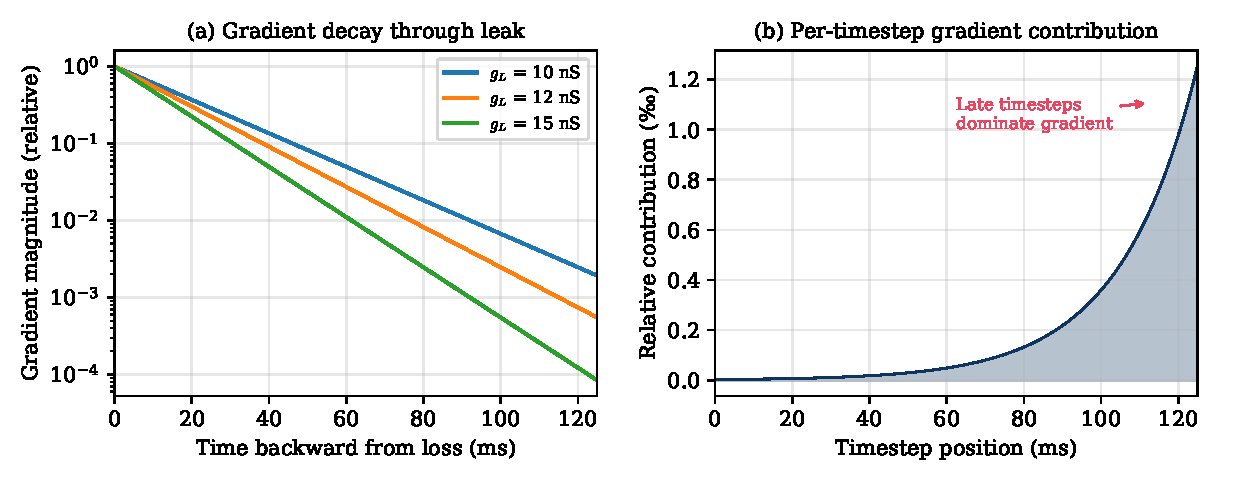
\includegraphics[width=0.95\textwidth]{figures/vanishing-gradients.pdf}
  \end{center}
  \caption{Vanishing gradients through leak dynamics. (a) Gradient magnitude decays exponentially as it propagates backward from the loss, shown for three leak conductance values
  $g_L$. (b) Consequence for per-timestep gradient contribution: early timesteps contribute negligibly to the total gradient, while the final milliseconds dominate.
  Computed for $g_L = 10$ nS, $C = 200$ pF, $dt = 0.025$ ms.}\label{fig:vanishing-gradients}
\end{figure}

\subsection{Surrogate gradients}\label{sec:bg:sg:surrogate-gradients}

There are a variety of surrogate functions that have been proposed.
The simplest one is the sigmoid function
\begin{equation}
  \sigma'(x) = \beta \cdot \sigma(\beta x)(1 - \sigma(\beta x)).
  \label{eq:sigmoid-surrogate}
\end{equation}
Other common surrogates include the exponential
\begin{equation}
  \sigma'(x) = \beta \cdot \exp(-\beta|x|)
  \label{eq:exponential-surrogate}
\end{equation}
and SuperSpike\cite{Zenke2018}
\begin{equation}
  \sigma'(x) = 1/(\beta|x| + 1)^2
  \label{eq:superspike-surrogate}
\end{equation}
functions.
All are centred at the discontinuity and unimodal, but differ in tail behaviour (Figure~\ref{fig:surr_grads}).

\begin{figure}
  \begin{center}
    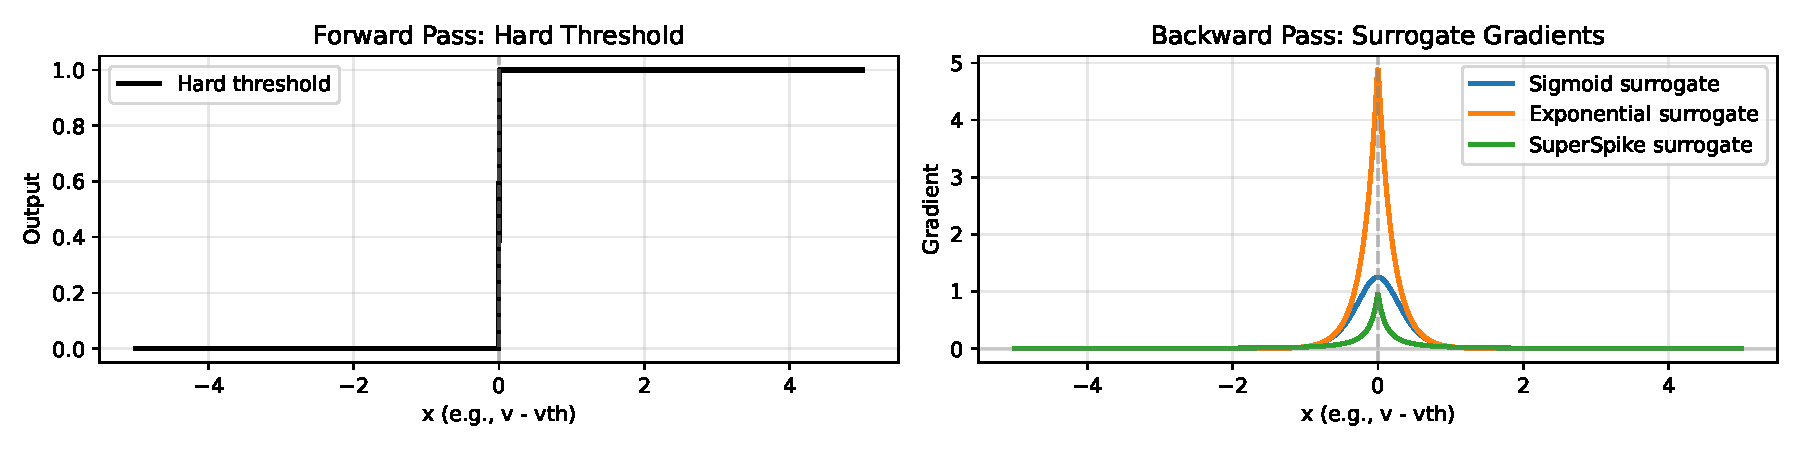
\includegraphics[width=0.95\textwidth]{figures/surrogate_gradients_comparison.pdf}
  \end{center}
  \caption{Surrogate gradient shape comparison. (a) The Heaviside step function used in the forward pass, with zero derivative everywhere except at the discontinuity. (b) Three
  common surrogate derivatives used in the backward pass: sigmoid, exponential, and SuperSpike. All are centered at the threshold and unimodal, but differ in peak height
  and tail decay. The steepness parameter $\beta$ (here $\beta = 5$) controls the width of the effective gradient window.}\label{fig:surr_grads}
\end{figure}

An important hyperparameter is the steepness $\beta$:
large $\beta$ concentrates the gradient signal in a narrow window around threshold, while small $\beta$ spreads it over a wider voltage range.
Gygax \& Zenke \cite{Gygax2025} show that surrogate gradients do not need to be the true gradient --- it is enough to only point in a useful descent direction.

We will further discuss the choice of surrogate, its steepness and how it interacts with the loss landscape in Section~\ref{}.\mtodo{update this once the section numbers are correct}

\section{Loss Functions for Spiking Models}\label{sec:bg:loss-functions}

Surrogate gradients allow gradients to flow backward in time, however, the loss function's landscape determines the direction of the gradient.
If the gradient points towards a non-spiking solution, the model will not produce correct spiking behaviour, no matter the surrogate gradient.

\subsection{Non-convex Parameter Space}\label{sec:bg:loss:param-space}
\itodo{Include plots of parameter space.}
The AdEx parameter space is highly non-convex.
Bifurcations in the dynamics --- the boundaries between non-spiking, tonic, and bursting regimes characterised by Naud et al.~\cite{Naud2008} --- mean that small parameter changes can cause large qualitative changes in firing behaviour.
A typical loss landscape therefore consists of large plateaus, on which the model is silent and the loss is insensitive to most parameters, separated by narrow valleys containing the spike-producing parameter combinations.
Gradient descent is consequently sensitive to initialisation: a starting point on a non-spiking plateau provides no gradient signal pointing towards the spike-producing region.

\subsection{Loss function categories}\label{sec:bg:loss:categories}
We can differentiate in three category of losses:
\begin{enumerate}
  \item Pointwise differences
  \item Feature-based losses
  \item Distance-based metrics
\end{enumerate}
Category one includes \gls{MSE}, \gls{MAE} and other variations.
\gls{MSE} is defined as
\begin{equation}\label{eq:MSE}
    \mathcal{L}_{\text{MSE}}(\theta) = \frac{1}{T} \sum_{t=1}^{T} \left( V_{\text{sim}}(t; \theta) - V_{\text{exp}}(t) \right)^2,
\end{equation}
where $\theta$ denotes the trainable parameters.

Usually these types of losses build a good starting point for lots of machine learning tasks, however, not in this case.
Consider two voltage traces with identical spiking frequencies but small temporal misalignments.
At each spike in one voltage trace, the other is in subthreshold regime.
This leads to high pointwise differences and therefore to high pointwise losses.
The crucial problem here is that a non spiking model would produce a smaller loss than the slightly misaligned one,
the gradient therefore pulls the model into non-spiking behaviour (see Section~\ref{sec:}\mtodo{fix this once section labels are done}, Figure~\ref{fig:mse-training-results})

The second category of loss functions are feature-based losses.
Here we evaluate the spike trains for different metrics, e.g. the number of spikes, spiking frequency, time to first spike, mean sub-threshold voltage or many more.
The simplest one is voltage mean and deviation, but they can be more specific.
These loss functions are commonly used for parameter fitting in simplified neuron models.
However, by default, most of these features are not in itself differentiable.
For non-gradient methods like Grid Search, Nelder-Mead or Genetic Algorithms, this is irrelevant.
When applied to gradient-based optimisations, possibly adjustments have to be made.
For example, the $\max$ function might be substituted with a $\text{softmax}$ alternative, which is defined as $\text{softmax}(z) \in (0, 1)^K$
\begin{equation}\label{eq:softmax}
  \text{softmax}(z)_i = \frac{e^{\beta z_i}}{\sum_{j=1}^K e^{\beta z_j}}
\end{equation}
for a tuple $\mathbf{z} = (z_1, ..., z_K) \in \mathbb{R}^K$ and a temperature $\beta \in \mathbb{R}^+$.
Also important to note is the fact that when different features are combined in a single loss, weighting each features contribution becomes another hyperparameter in the training process.

The third category contains spike-train similarity metrics such as the Van Rossum distance and dynamic time warping.
Unlike MSE, these compare spike trains as structured objects rather than sample-by-sample;
unlike feature-based losses, they preserve the full temporal structure of the train.

The Van Rossum distance \cite{Rossum2001} convolves each spike train with a causal exponential kernel $K(t) = \exp(-t/\tau)$ and computes the $L^2$ distance between the resulting filtered traces:
\begin{equation}\label{eq:van-rossum}
    \mathcal{L}_{\text{VR}}^2 = \frac{1}{\tau} \int_0^T \left( f_{\text{sim}}(t) - f_{\text{exp}}(t) \right)^2 dt
\end{equation}\mwarning{Alex wrote $t_i > t?$ here, I'm unsure what that means...}
where $f(t) = \sum_i K(t - t_i)$ is the filtered spike train.
The time constant $\tau$ controls the temporal precision: small $\tau$ penalises sub-millisecond timing errors (temporal coding),
while large $\tau$ smooths over individual spikes and compares overall firing rates (rate coding).
Because convolution and the $L^2$ norm are smooth operations, the Van Rossum distance is naturally differentiable --- no special treatment is required for the loss itself.

An alternative approach is Dynamic Time Warping (DTW) \cite{Sakoe1978}, which finds an optimal alignment between two time series by warping the time axis.
Given two sequences $x \in \mathbb{R}^n$ and $y \in \mathbb{R}^m$ with pointwise cost matrix $\delta_{i,j} = (x_i - y_j)^2$, the DTW distance is defined via the recursion
\begin{align}\label{eq:dtw}
    r_{i,j} &= \delta_{i,j} + \min\!\left( r_{i-1,j-1},\; r_{i-1,j},\; r_{i,j-1} \right),\nonumber\\
    \mathcal{L}_{\text{DTW}}(x, y) &= r_{n,m},
\end{align}
with boundary conditions $r_{0,0} = 0$ and $r_{i,0} = r_{0,j} = \infty$ for $i, j > 0$.
Unlike pointwise losses, DTW tolerates temporal shifts by design; however, the hard minimum in Eq.~\eqref{eq:dtw} is not differentiable.
Soft-DTW \cite{Blondel2018} replaces it with the softmin
\begin{equation}\label{eq:softmin}
    \min{}^{\gamma}(a_1, \dots, a_k) = -\gamma \log \sum_{i=1}^{k} \exp(-a_i / \gamma),
\end{equation}
yielding the smoothed recursion
\begin{align}\label{eq:soft-dtw}
    r_{i,j}^{\gamma} &= \delta_{i,j} + \min{}^{\gamma}\!\left( r_{i-1,j-1}^{\gamma},\; r_{i-1,j}^{\gamma},\; r_{i,j-1}^{\gamma} \right),\nonumber\\
    \mathcal{L}_{\text{SDTW}}^{\gamma}(x, y) &= r_{n,m}^{\gamma}.
\end{align}
The smoothing factor $\gamma > 0$ controls the relaxation:
as $\gamma \to 0$, Soft-DTW recovers the original DTW distance, while larger $\gamma$ produces smoother gradients at the cost of a looser alignment.\footnote{This is the equivalent to the inverse temperature $\beta$ from the softmax function (eq.~\ref{eq:softmax})}
This makes the alignment distance amenable to gradient-based optimisation, at the cost of $O(nm)$ time and memory complexity.

All three categories share one fundamental constraint: every operation in the computational path from parameters to loss must be differentiable.
For pointwise losses, this is trivially satisfied.
For feature-based losses, operations like spike detection and counting must be replaced with soft, differentiable approximations.
For distance metrics operating on spike trains, the spike train itself must be represented in a differentiable form.
This requirement ties directly back to the surrogate gradient framework introduced in Section~\ref{sec:bg:surrogate-gradients}:
the surrogate provides a soft spike indicator $s(t) \in [0, 1]$ that can serve as input to any of these loss functions.

\section{Summary}\label{sec:bg:summary}
The AdEx model provides an efficient yet expressive neuron model, but parameters must be fitted through optimisation to get expressive, neuron imitating firing behaviour.
Gradient-based methods are attractive due to their computational efficiency, however, the Heaviside reset mechanism creates a differentiability barrier that prevents standard automatic differentiation.
Surrogate gradients restore gradient flow through spike events by replacing the Heaviside derivative with a smooth surrogate during the backward pass.
Three challenges remain: the parameter space is highly non-convex, gradients still decay exponentially through the leak dynamics, and the surrogate steepness $\beta$ must be chosen carefully.
The loss function is equally critical.
MSE on raw voltage traces drives the optimiser towards non-spiking solutions, feature-based losses lack temporal credit assignment, and distance metrics like Van Rossum or soft-DTW offer promising alternatives but come with their own trade-offs.
The interplay between surrogate choice and loss function design is the central challenge investigated in this work.
